\section{Il Modello \textit{\textit{airgun}NoiseEstimation}}

Il modello \textbf{\textit{airgun}NoiseEstimation} simula la propagazione del rumore generato da un \textit{\textit{airgun}} sottomarino e produce una mappa dell'inquinamento acustico marino nella zona di studio.

L'obiettivo del modello è stimare come il rumore emesso da un \textit{\textit{airgun}}, ossia una sorgente impulsiva ad alta potenza usata nelle prospezioni sismiche, si propaghi nell'ambiente marino, producendo una mappa spaziale dei livelli sonori (in dB) attorno alla sorgente.

\subsection{Fasi del processo di simulazione}

\begin{enumerate}
  \item \textbf{Definizione dell'area di studio}, tipicamente un cerchio centrato sull'\textit{\textit{airgun}} con raggio prestabilito (es. 1000 km).
  \item \textbf{Suddivisione in settori radiali}: l'area viene suddivisa in \(N\) spicchi (es. 90) per valutare radialmente la propagazione.
  \item \textbf{Simulazione della propagazione lungo ciascun settore}, considerando:
    \begin{itemize}
      \item batimetria e morfologia del fondale;
      \item rotte navali che possono influenzare la diffusione;
      \item profili di velocità del suono (\textit{sound speed profiles});
      \item ostacoli naturali come coste e isole.
    \end{itemize}
  \item \textbf{Calcolo dei livelli di rumore} lungo ogni linea radiale, in \(\mathrm{dB_{SPL}}\). Questa unità di misura rappresenta il livello di pressione sonora. È una misura logaritmica della pressione acustica relativa a un valore di riferimento, usato per quantificare l'intensità del suono. \cite{db-spl-definition}
  \item \textbf{Assemblaggio della mappa finale}, combinando tutti i settori in un dataset \textit{geoposizionato}.
\end{enumerate}

\subsection{Output generati}

Il modello produce un file contenente coordinate GPS, livelli di pressione sonora e informazioni ambientali. In particolare, i dati presenti sono i seguenti:

\begin{itemize}
  \item coordinate GPS dei punti campionati;
  \item livelli di rumore in dB;
  \item dati ambientali (profondità, distanza dalla sorgente);
  \item etichette di settore per ogni punto.
\end{itemize}

Questi dati possono essere elaborati ulteriormente con il fine di visualizzare i dati contenuti sotto forma di rappresentazioni grafiche significative. Il mio contributo al progetto si è focalizzato su quest'ultimo aspetto, ossia rappresentare decine di migliaia di \textit{datapoints} su una mappa digitale, permettendo un'interazione dinamica. Si veda un esempio di rappresentazione grafica in Figura \ref{fig:preview-heatmap}.

\begin{figure}
    \centering
    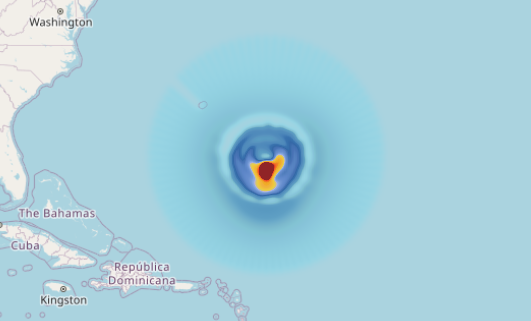
\includegraphics[width=0.75\linewidth]{images/heatmap.png}
    \caption{Visualizzazione dei dati generati su mappa (HeatMap)}
    \label{fig:preview-heatmap}
\end{figure}

Una breve anteprima dei dati testuali generati:

\begin{table}[ht]
\centering
\label{tab:data}
\begin{tabular}{
    S[table-format=2.15]
    S[table-format=-2.1]
    S[table-format=2.15]
    S[table-format=4.0]
    S[table-format=4.15]
    S[table-format=1.1]
}
\toprule
{Latitude} & {Longitude} & {Value} & {Bathy1} & {Bathy2} & {Sector} \\
\midrule
37.25897980148502 & -59.3 & 88.04606789424417 & 1003 & 5163.03076171875  & 0.0 \\
37.24995686563234 & -59.3 & 88.04978137920247 & 2007 & 5167.09033203125  & 0.0 \\
37.24093392977967 & -59.3 & 88.05349035487939 & 3011 & 5166.5244140625   & 0.0 \\
37.231910993927   & -59.3 & 88.05719509329765 & 4015 & 5166.5576171875   & 0.0 \\
37.22288805807432 & -59.3 & 88.06089653237328 & 5019 & 5166.21142578125  & 0.0 \\
37.21386512222165 & -59.3 & 88.06459277272671 & 6022 & 5161.037109375    & 0.0 \\
37.20484218636896 & -59.3 & 88.06828474014407 & 7026 & 5158.3720703125   & 0.0 \\
\bottomrule
\end{tabular}
\end{table}

\subsection{Utilità principale}

I risultati generati dal modello permettono di stimare con precisione le aree di maggiore impatto acustico attorno alla sorgente, evidenziando come il rumore si attenui con la distanza seguendo le leggi della propagazione sott'acqua. \cite{airgun_marine_life} 
Grazie all'inclusione di rotte navali e dettagli morfologici come isole, coste e batimetria, il modello è in grado di identificare zone con livello di rumore più elevato e zone \say{ombra} dove il suono è attenuato rispetto all'ambiente circostante.

\noindent In sintesi, il modello trasforma una simulazione fisica complessa in un output geografico e operativo, utile per la gestione responsabile dell'inquinamento acustico marino.
